\documentclass[landscape]{article}
\usepackage[pdftex]{graphicx,color}
\usepackage{amssymb}
\pagestyle{empty}
\oddsidemargin  -0.5 in
\evensidemargin -0.5 in
\headheight     0 in
\topmargin      -1 in
\textheight     7.7 in
\textwidth      10 in
\newenvironment{slide}[1][ ]{\mbox{\bf #1 } \vfill}{\vfill \mbox{ } \hfill \Large \arabic{page} \pagebreak}
\begin{document}
\Huge \sffamily
\renewcommand{\labelitemi}{{\LARGE $\stackrel{\bullet}{\mbox{ }}$}}
\setlength{\parindent}{0 cm}

\begin{slide}
\begin{center}
Electron Identification without the Pixel Detector

\vspace{0.5 cm}
First Progress Report

\vspace{1.5 cm}
Jim Pivarski

\vspace{0.25 cm}
Cornell University
\end{center}
\end{slide}

\begin{slide}
Outline for this talk

\vspace{1 cm}
\begin{itemize}\setlength{\itemsep}{1 cm}

\item Project outline and goals (part of the project was to define it)

\item Pixel algorithm and why $e^\pm$-finding is harder without a pixel detector

\item The importance of realistic Monte Carlo

\item Implementing a placeholder in CMSSW

\item Next steps

\end{itemize}
\end{slide}

\begin{slide}
Project Outline and Goals (we welcome corrections)

\vspace{0.5 cm}
\begin{center}
\begin{minipage}{0.85\linewidth}

{\bf Goal:} identify electrons (HLT and offline) and reject
background by matching ECAL SuperClusters to Si-strip tracker hits

\vspace{0.5 cm}
\begin{center}
\begin{minipage}{0.85\linewidth}
A well-studied algorithm exists which matches SuperClusters to pixel hits

\vspace{0.5 cm} Early data will be taken without a complete pixel
detector, so our algorithm is a fallback
\end{minipage}
\end{center}

\vspace{1 cm}
{\bf Strictly Level 2.5:} input is reconstructed SC and tracker hits, output is
\begin{itemize}

\item a list of electron candidate objects {\it for HLT filter to save event if non-empty}

\item track parameters {\it to seed a track in Level 3}

\item possibly other quality objects (list of hits, not for seeding)

\end{itemize}

\end{minipage}
\end{center}
\end{slide}

\begin{slide}
Project Goals (continued)

\vspace{1 cm}
\begin{description}

\item[fast:] $\lesssim$100 ms per SuperCluster on a 1~GHz PC

scale as a low power of background hits: $\mathcal{O}(\mbox{hits}\,^p)$ where $p \lesssim 2$

\vspace{1 cm}

\item[robust:] electron-finding efficiency independent of tracker misalignments of $\sim$500~$\mu$m,

independent of tracker-ECAL misalignments of $\sim$1~mm, and

independent of number of background hits

($\rightarrow$~this will make electron efficiency easier to understand)

\vspace{1 cm}

\item[flexible:] provide parameters to tune efficiency versus rejection, and/or versus speed

\end{description}
\end{slide}

\begin{slide}
Pixel Algorithm

\vspace{0.5 cm}
\begin{enumerate}

\item Project helix from ECAL position to origin (curvature from SC energy)

for each of two charge hypotheses

\item Wide window in first pixel layer; identified hit narrows search
window on subsequent layers

\end{enumerate}

\vspace{0.5 cm}
Electrons radiate in tracker material and often intersect ECAL far
from initial helix.  {\it Why does a helix projection work?}

\vspace{0.5 cm}
\begin{center}
\begin{tabular}{p{0.45\linewidth} p{0.45\linewidth}}
\begin{minipage}{\linewidth}
{\bf Theorem:} if all bremsstrahlung photons are included in a SC,
energy-weighted position is on the initial helix

\vspace{0.5 cm}
{\bf Lesson:} inner hits point more reliably to SC position

\end{minipage} &
\begin{minipage}{\linewidth}
\begin{center}
\mbox{\hspace{1 cm}} 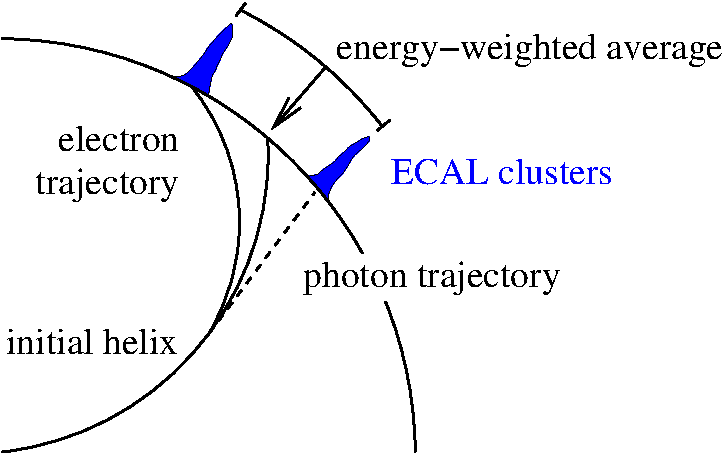
\includegraphics[width=\linewidth]{theorem} \mbox{\hspace{-1 cm}}
\end{center}
\end{minipage}
\end{tabular}
\end{center}
\end{slide}

\begin{slide}
Pixel algorithm performance

(something to aim for without being too expectant)

\vspace{1 cm}

\begin{center}
\begin{tabular}{p{0.45\linewidth} p{0.45\linewidth}}
\begin{minipage}{\linewidth}
\begin{center}
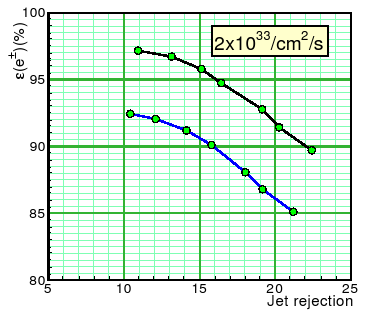
\includegraphics[width=\linewidth]{pixel_performance}
\end{center}
\end{minipage} &
\begin{minipage}{\linewidth}

Pixel's advantage: $Z$ precision

$\Delta Z$ cut window = 1~mm

\vspace{1 cm}

Tracker has 4 stereo layers with 1~mm resolution

\vspace{0.5 cm}

but most layers have only 10--20~cm segmentation in $Z$

\vspace{1 cm}
Try to regain lost signal/noise by looking for more than 3 hits

\end{minipage}
\end{tabular}
\end{center}

\vspace{1 cm}
(We'd like to make the equivalent plot, but need the same MC samples)
\end{slide}

\begin{slide}
``Event Displays''

\vspace{1 cm}

vertical axis is $\phi$ position of each hit with SuperCluster's $\phi$ as zero

horizontal axis is cylindrical radius of each hit

\begin{center}
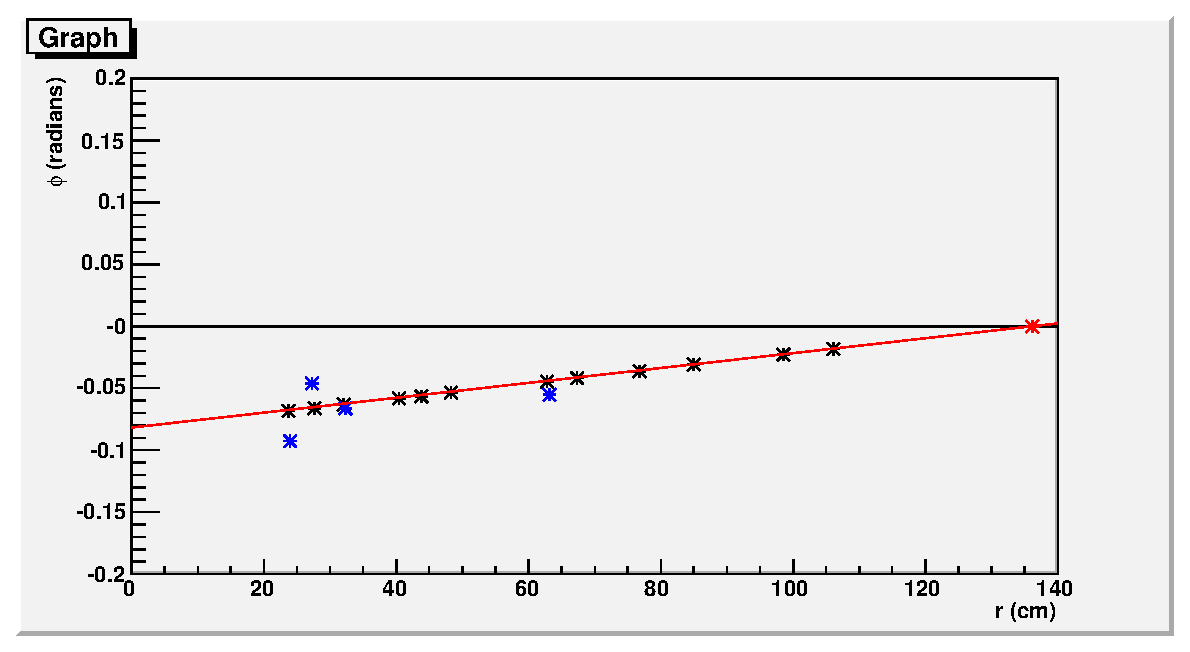
\includegraphics[width=0.75\linewidth]{event_display}
\end{center}

\vspace{1 cm}
helical track projects an arcsin curve, but even at 10~GeV, this is linear

(helix is approximated by a parabola)

\end{slide}

\begin{slide}
A typical electron

\vspace{1 cm}
\begin{center}
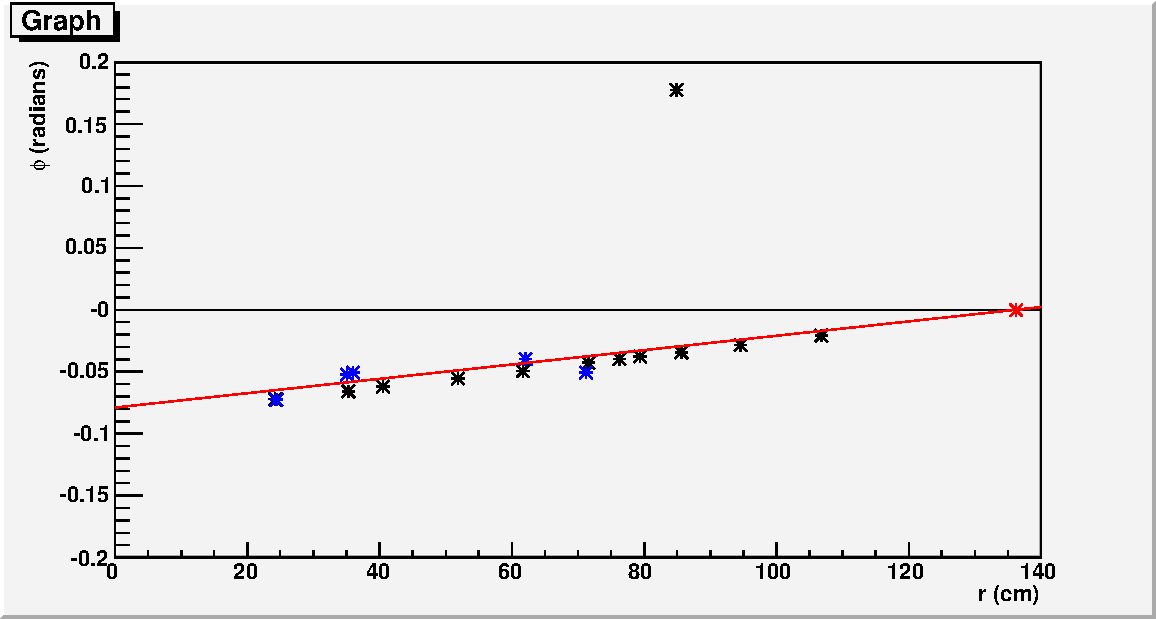
\includegraphics[width=\linewidth]{event_display_typical}
\end{center}
\end{slide}

\begin{slide}
  Electron with early scatter or bremsstrahlung ({\it not} in pixel material!)

\vspace{1 cm}
\begin{center}
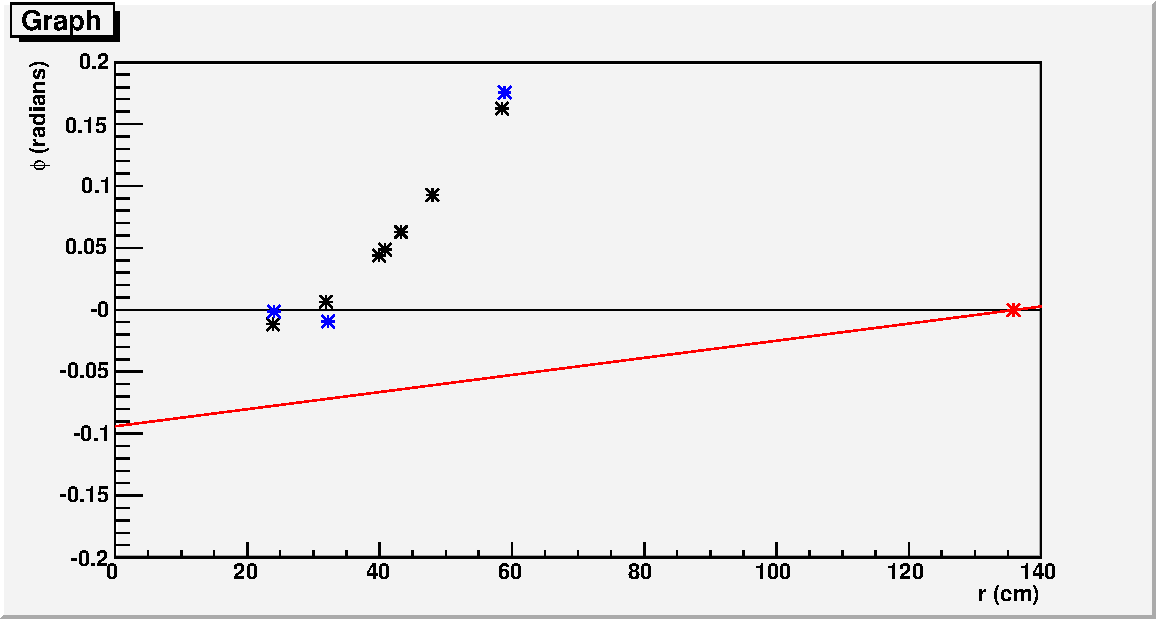
\includegraphics[width=\linewidth]{event_display_scatterearly}
\end{center}
\end{slide}

\begin{slide}
Electron with scatter in strip tracker

\vspace{1 cm}
\begin{center}
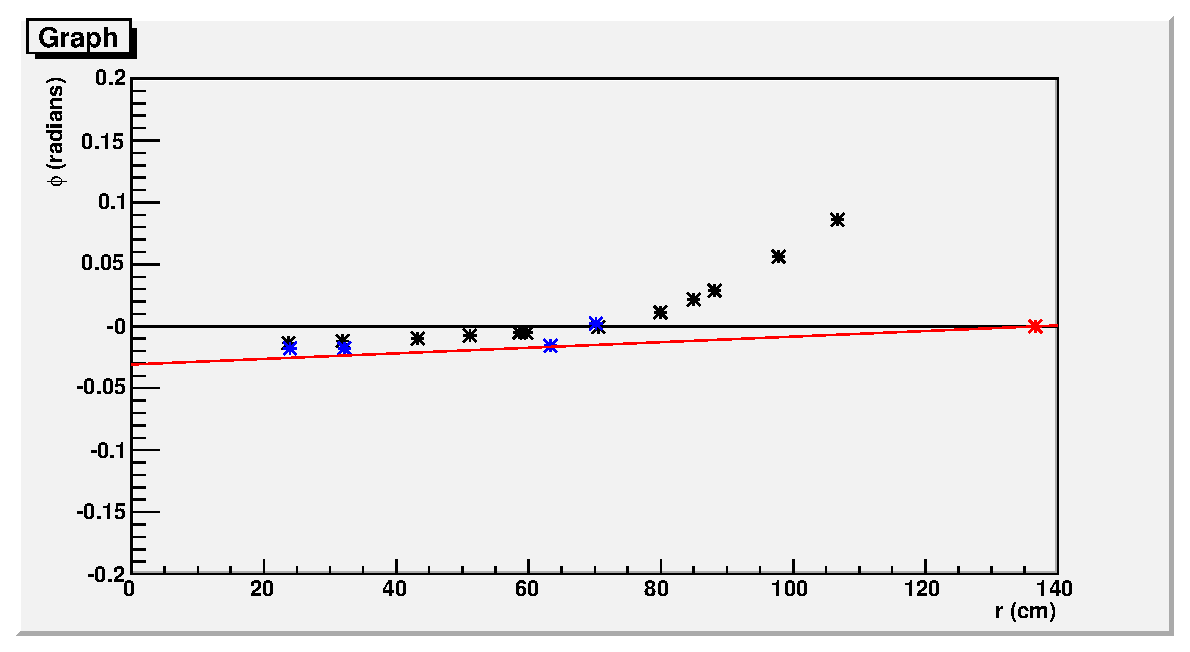
\includegraphics[width=\linewidth]{event_display_scattersi2}
\end{center}
\end{slide}

\begin{slide}
Electron with wrong SuperCluster position (lost a photon?)

\vspace{1 cm}
\begin{center}
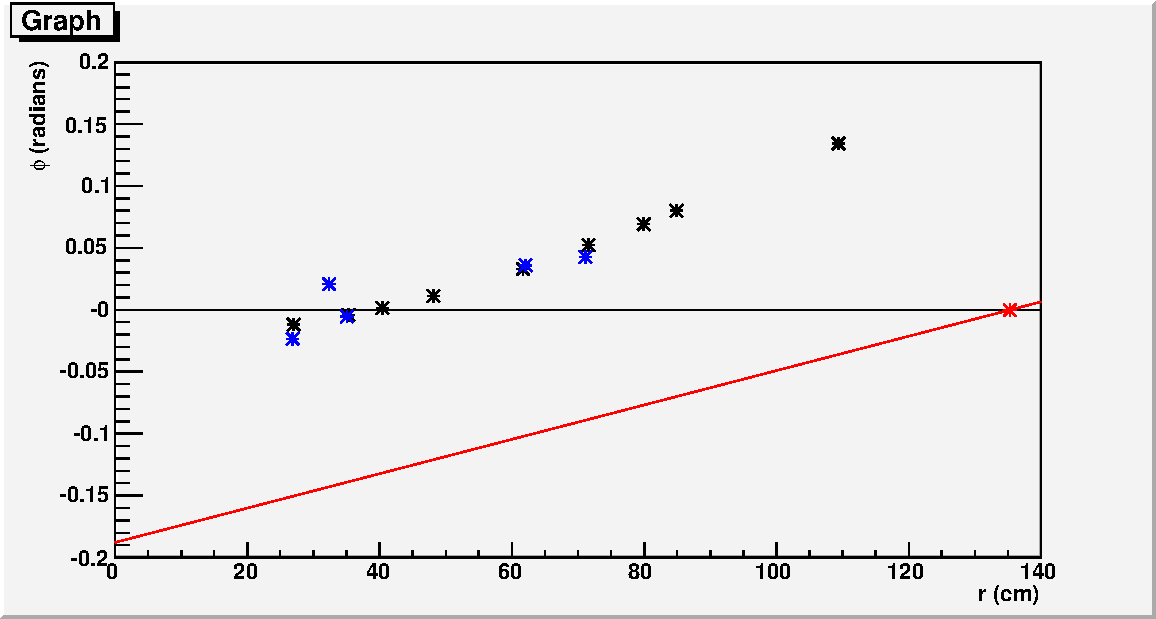
\includegraphics[width=\linewidth]{event_display_wrongsc}
\end{center}
\end{slide}

\begin{slide}
A typical electron superimposed on minbias (to simulate underlying event)

\vspace{1 cm}
\begin{center}
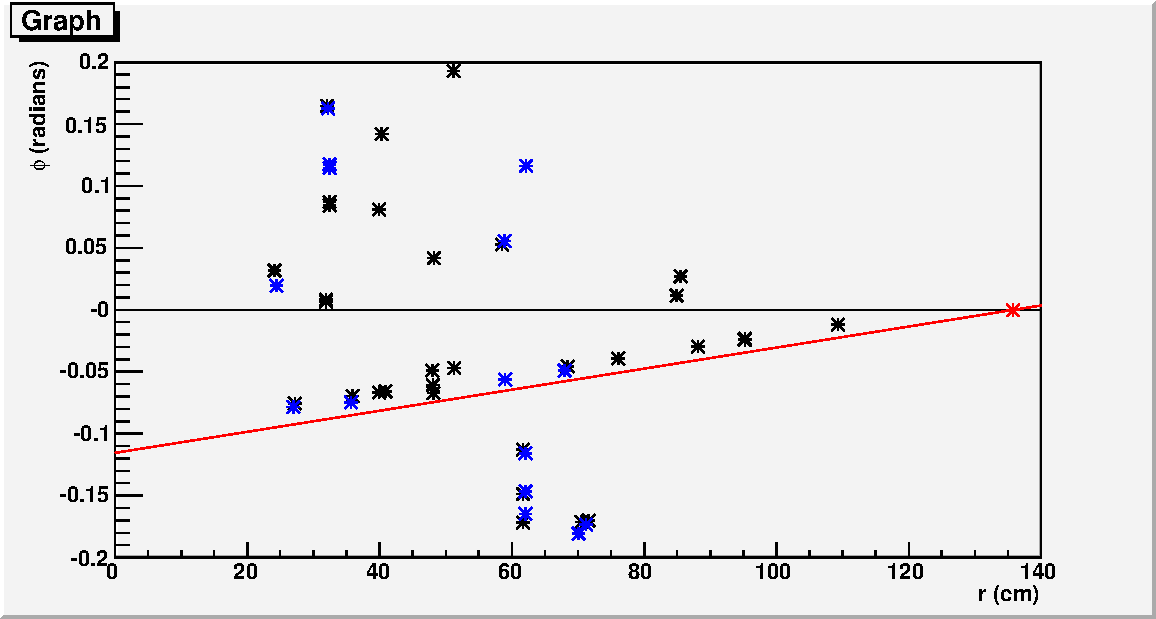
\includegraphics[width=\linewidth]{event_display_superimposed}
\end{center}
\end{slide}

\begin{slide}
Background: minbias event \underline{with a 17~GeV SuperCluster} % 17.8 GeV

\vspace{1 cm}
\begin{center}
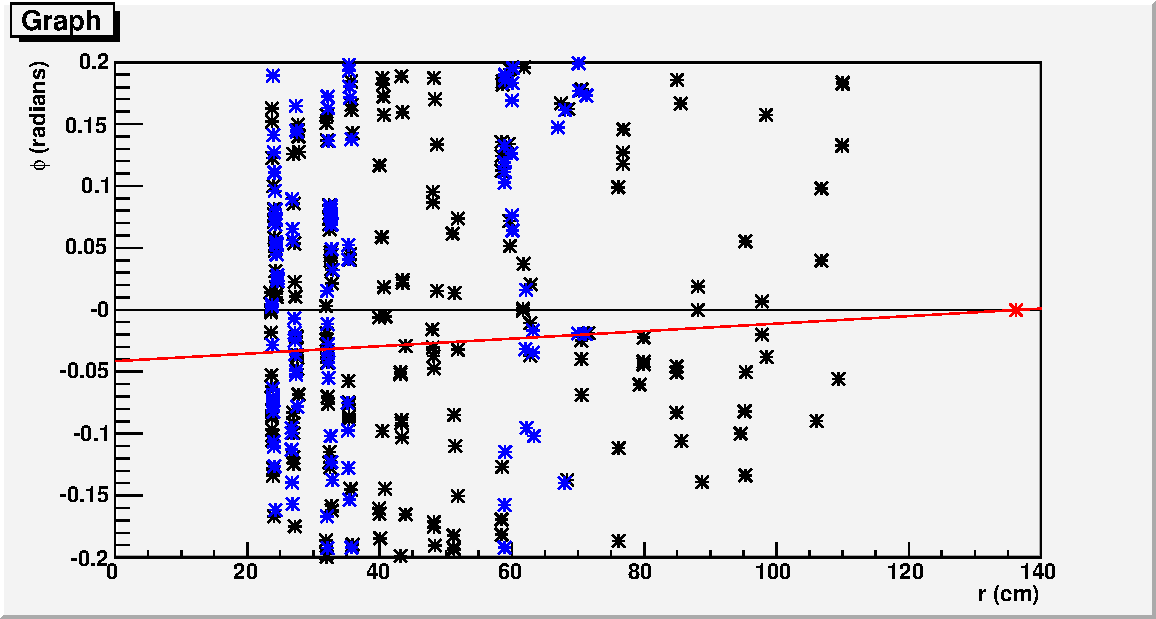
\includegraphics[width=\linewidth]{event_display_background}
\end{center}
\end{slide}

\begin{slide}
Here's a simple algorithm:

\vspace{0.5 cm}
Define a 10~mrad $\Delta \phi$ band around hypothesis, count hits within that band

\vspace{1 cm}
\begin{center}
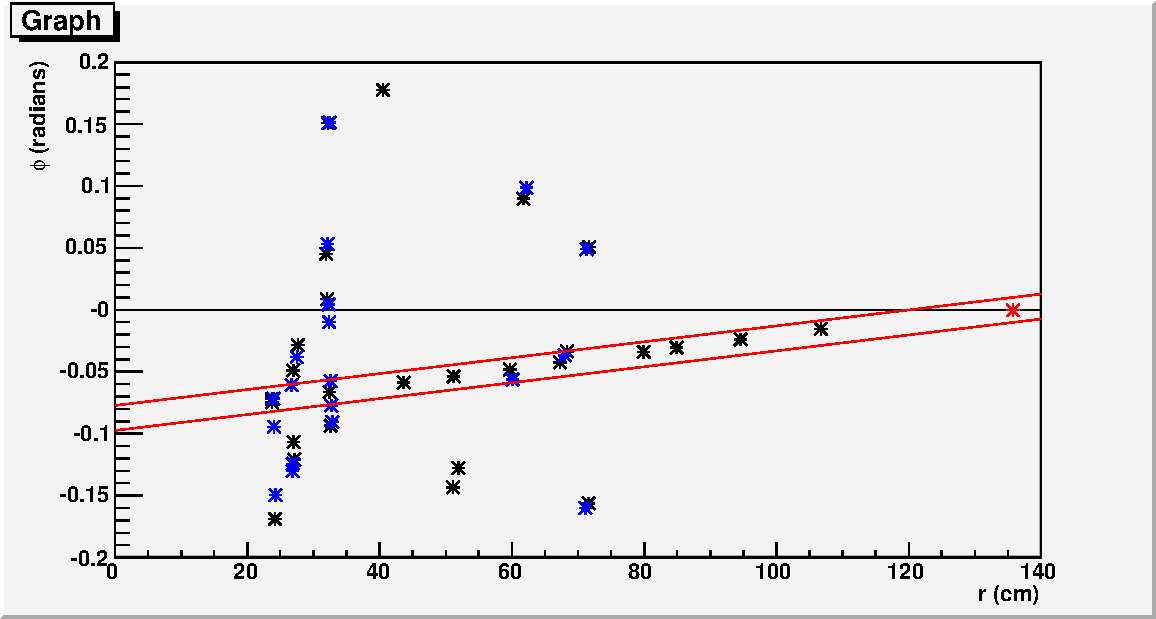
\includegraphics[width=\linewidth]{event_display_banded}
\end{center}
\end{slide}

\begin{slide}
Where to set minimum number of hits cut?

\vspace{0.25 cm}
\begin{center}
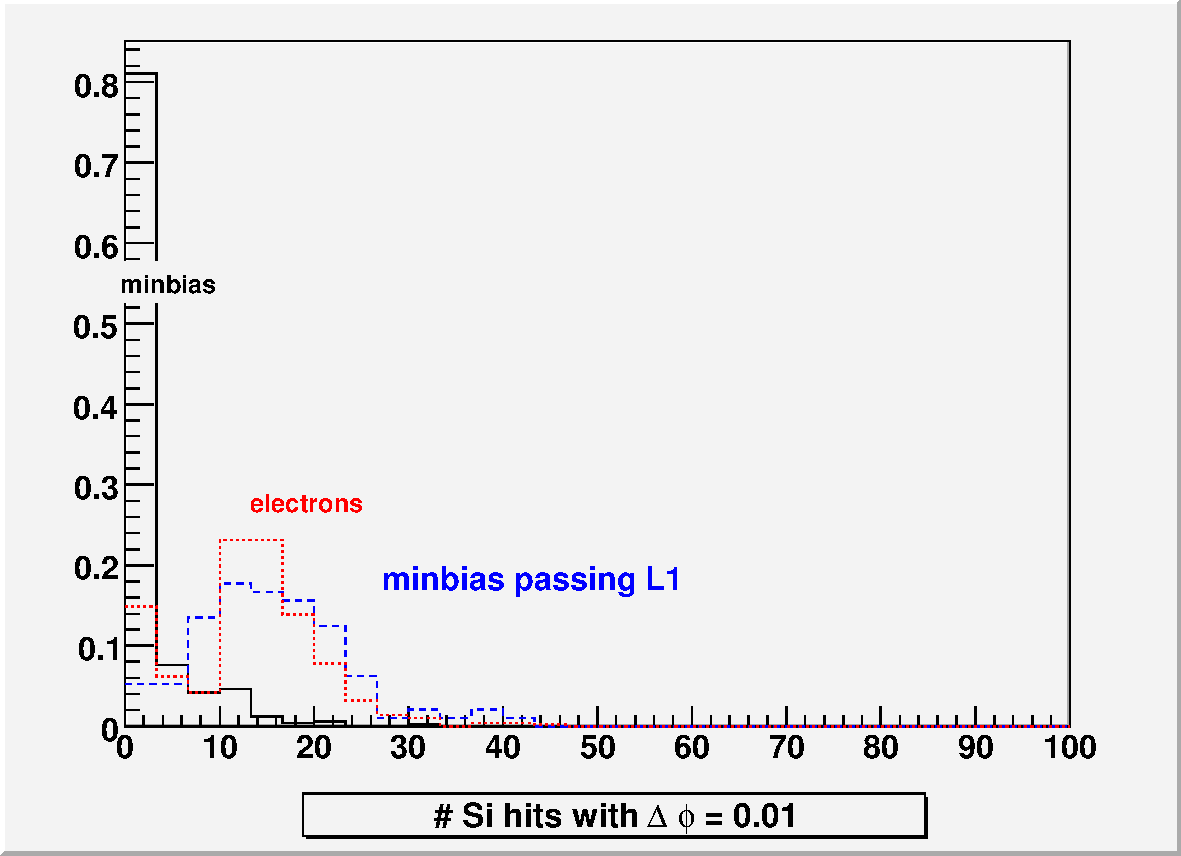
\includegraphics[width=0.7\linewidth]{hitdistributions}
\end{center}

\vspace{0.5 cm}
\textcolor{blue}{minbias passing L1} ($\ge$~17~GeV SC) is staring into a jet for most events
\end{slide}

\begin{slide}
Narrow $\Delta \phi$ to 2~mrad?

\vspace{0.25 cm}
\begin{center}
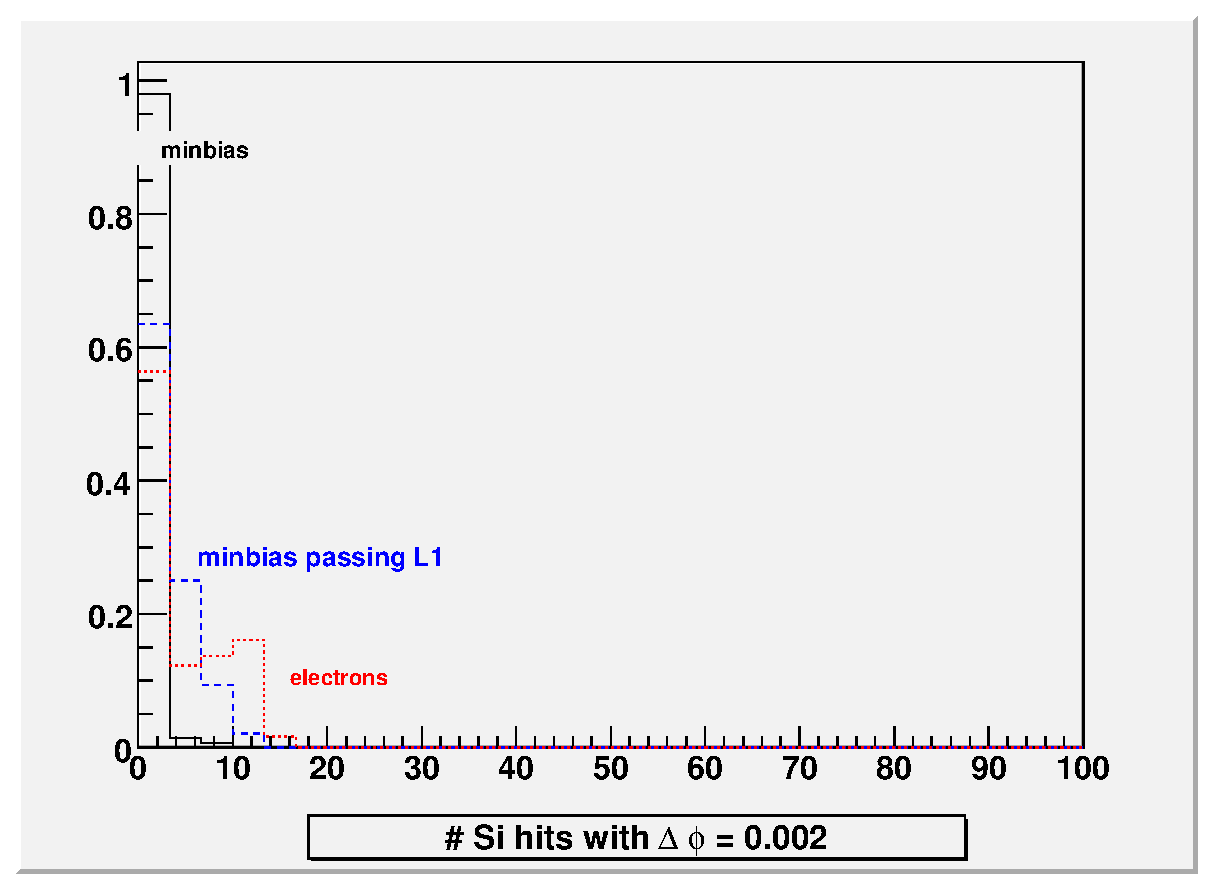
\includegraphics[width=0.7\linewidth]{hitdistributions_narrow}
\end{center}

\vspace{0.5 cm}
Not narrow enough to distinguish electrons from background,

and too narrow for robustness goals
\end{slide}

\begin{slide}
Widen $\Delta \phi$ to 100~mrad and cut on {\it maximum} number of hits?

\begin{center}
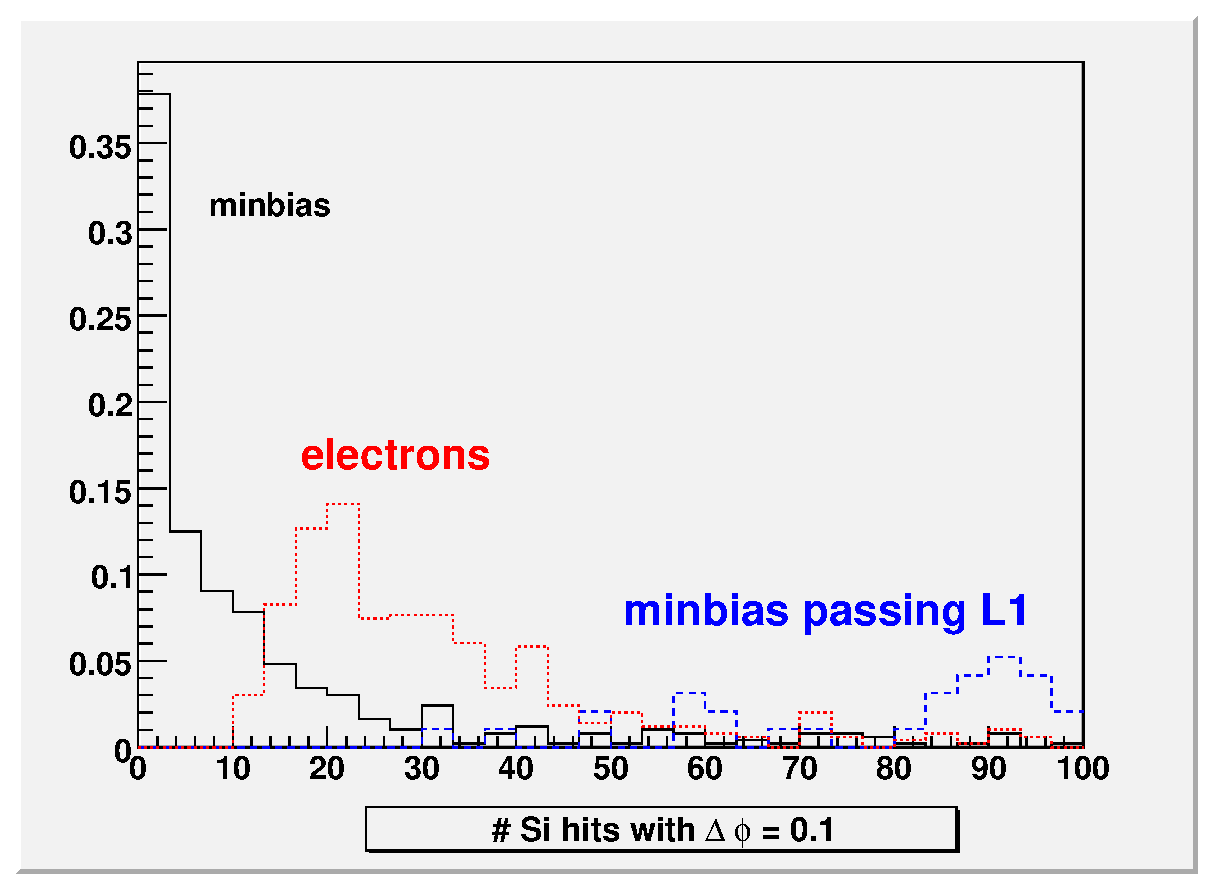
\includegraphics[width=0.65\linewidth]{hitdistributions_wide}
\end{center}

That would be a track isolation cut, not track-cluster matching!

Can we afford to isolate electons?  Need to see physics electrons.

\vspace{0.25 cm}
\begin{center}
\textcolor{blue}{\fbox{MC studies drive algorithm development}}
\end{center}
\end{slide}

\begin{slide}
Nevertheless, we will implement a placeholder in CMSSW.

\vspace{1 cm}
Proposal:

\vspace{0.5 cm}
\begin{center}
\begin{minipage}{0.9\linewidth}
\begin{itemize}

\item add {\tt SiStripElectronCandidate} to {\tt EgammaCandidates}

\vspace{0.5 cm}
\begin{center}
\begin{minipage}{0.9\linewidth}
as a subclass of {\tt ElectronCandidate}

\vspace{0.5 cm}
(sibling of {\tt PixelElectronCandidate}?)
\end{minipage}
\end{center}

\vspace{1 cm}
\item add {\tt SiStripElectronProducer} to {\tt RecoEcal}

\vspace{1 cm}
\item add {\tt ElectronCandidateAnalyzer} to {\tt RecoEcal}
\end{itemize}
\end{minipage}
\end{center}

\vspace{1 cm}
Algorithm will be trivial (no background rejection) until we get more
information from physics studies

\end{slide}

\begin{slide}
Next steps:

\vspace{0.75 cm}
\begin{itemize}

\item Check approved subclass, producer, and analyzer into CVS (today)

\item Obtain realistic Monte Carlo

\begin{center}
\begin{minipage}{0.95\linewidth}
\begin{description}

\item[signal:] physics electrons (how often do they overlap jets?)

underlying event and multiple interactions at generator level

(how often do U.L.\ and M.I.\ interfere with stereo matching?)

remove pixel material (done)

\item[background:] large minbias sample which has passed Level 2

(we quickly generated our sample by requiring generator-level \mbox{\hspace{3 cm}} \hfill $p_T >$ 50~GeV)

This should be communal, right?  Does it exist?

\end{description}
\end{minipage}
\end{center}

\item Study event properties (in CMSSW/FWLite)

\hspace{4.5 cm} $\uparrow$ \hspace{0.5 cm} $\downarrow$

\item Improve algorithm (in CMSSW)

\end{itemize}
\end{slide}


\end{document}
